\documentclass[10pt,twocolumn]{IEEEtran}


% correct bad hyphenation here
\hyphenation{op-tical net-works semi-conduc-tor}

\usepackage{amsmath,graphicx,amsfonts,amssymb,amsthm,epsfig,mathrsfs,balance}
\usepackage{subcaption,tikz,color,multirow,algorithm,algpseudocode,algorithmicx}
\usepackage{cite,url,framed,bm,dsfont,lipsum}

\setlength{\tabcolsep}{1.1pt}

\newtheorem{assumption}{Assumption}
\newtheorem{theorem}{Theorem}
\newtheorem{corollary}[theorem]{Corollary}
\newtheorem{definition}{Definition}
\newtheorem{lemma}{Lemma}
\newtheorem{proposition}{Proposition}
\newtheorem{remark}{Remark}
\newtheorem{property}{Property}
\newtheorem{example}{Example}

\newcommand{\differential}{{\rm{d}}}

\renewcommand*{\thefootnote}{\fnsymbol{footnote}}
\newcommand{\red}{\color{red}}



\begin{document}

\title{\LARGE \bf Stochastic Uncertainty Propagation in Power System Dynamics using Measure-valued Proximal Recursions}

\author{Abhishek~Halder,~\IEEEmembership{Member,~IEEE,} Authors}
%\author{Abhishek~Halder,~\IEEEmembership{Member,~IEEE,}
%Xinbo~Geng,~\IEEEmembership{Member,~IEEE,}
%        Kenneth~F. Caluya,
%        and~Pegah~Ojaghi% <-this % stops a space
%\thanks{A. Halder and K.F. Caluya are with the Department of Applied Mathematics, University of California, Santa Cruz, CA 95064, USA, {\texttt{\{ahalder,kcaluya\}@ucsc.edu}}.}% <-this % stops a space
%\thanks{X. Halder is with the Department of Applied Mathematics, University of California, Santa Cruz, CA 95064, USA, {\texttt{\{ahalder\}@ucsc.edu}}. This research was partially supported by the NSF award 1923278.}}% <-this % stops a space
%\thanks{Manuscript received April 19, 2005; revised August 26, 2015.}}
% The paper headers
%\markboth{Journal of \LaTeX\ Class Files,~Vol.~14, No.~8, August~2015}%

\maketitle

\begin{abstract}
We present a proximal algorithm that performs a variational recursion on the space of joint probability measures to propagate the stochastic uncertainties in power system dynamics over high dimensional state space. The proposed algorithm takes advantage of the exact nonlinearity structures in the trajectory-level dynamics of the networked power systems, and is nonparametric. Lifting the dynamics to the space of probability measures allows us to design a scalable algorithm that obviates gridding the underlying high dimensional state space or function approximation. The proximal recursion implements a generalized gradient flow, and evolves probability weighted scattered point clouds. We provide the theoretical details, convergence guarantees, and numerical examples on realistic test systems.
\end{abstract}

\begin{IEEEkeywords}
Uncertainty propagation, power system dynamics, optimal transport, proximal operator.
\end{IEEEkeywords}



\section{Introduction}\label{sec:intro}
%\IEEEPARstart{T}{he} networked dynamics of electrical generators and loads include different types of uncertainties: intermittencies in renewable generation, load level random fluctuations, parametric uncertainties in transmission lines, uncertainties in weather, unexpected outages, noise in phasor measurement unit sensing data, among others. While significant progress has been made in statistically quantifying these individual sources of uncertainties, it remains challenging \cite{schwalbe2015mathematical} to accurately predict the joint effect of these uncertainties on the safe and robust operation of the power system over time.

%The study of power system dynamics with uncertainties is not new. However, 
\IEEEPARstart{S}{tochastic} variabilities in power grid have increased significantly in recent years both in the generation side (e.g., due to growing penetration of renewables) as well as in the load side (e.g., due to widespread adoption of plug-in electric vehicles). Several studies \cite{timko1983monte,nwankpa1992stochastic,odun2012structure,ghanavati2016identifying,apostolopoulou2016assessment} have reported that even small stochastic effects can significantly alter the assessment of transient stability, or the performance of automatic generation control. However, the lack of a rigorous yet scalable stochastic computational framework continues to impede \cite{schwalbe2015mathematical} our ability to perform transient analysis involving time varying joint probability density functions (PDFs) over the states of a large power system network. In this paper, we present a new algorithm to address this computational need.  

\begin{figure}
\centering
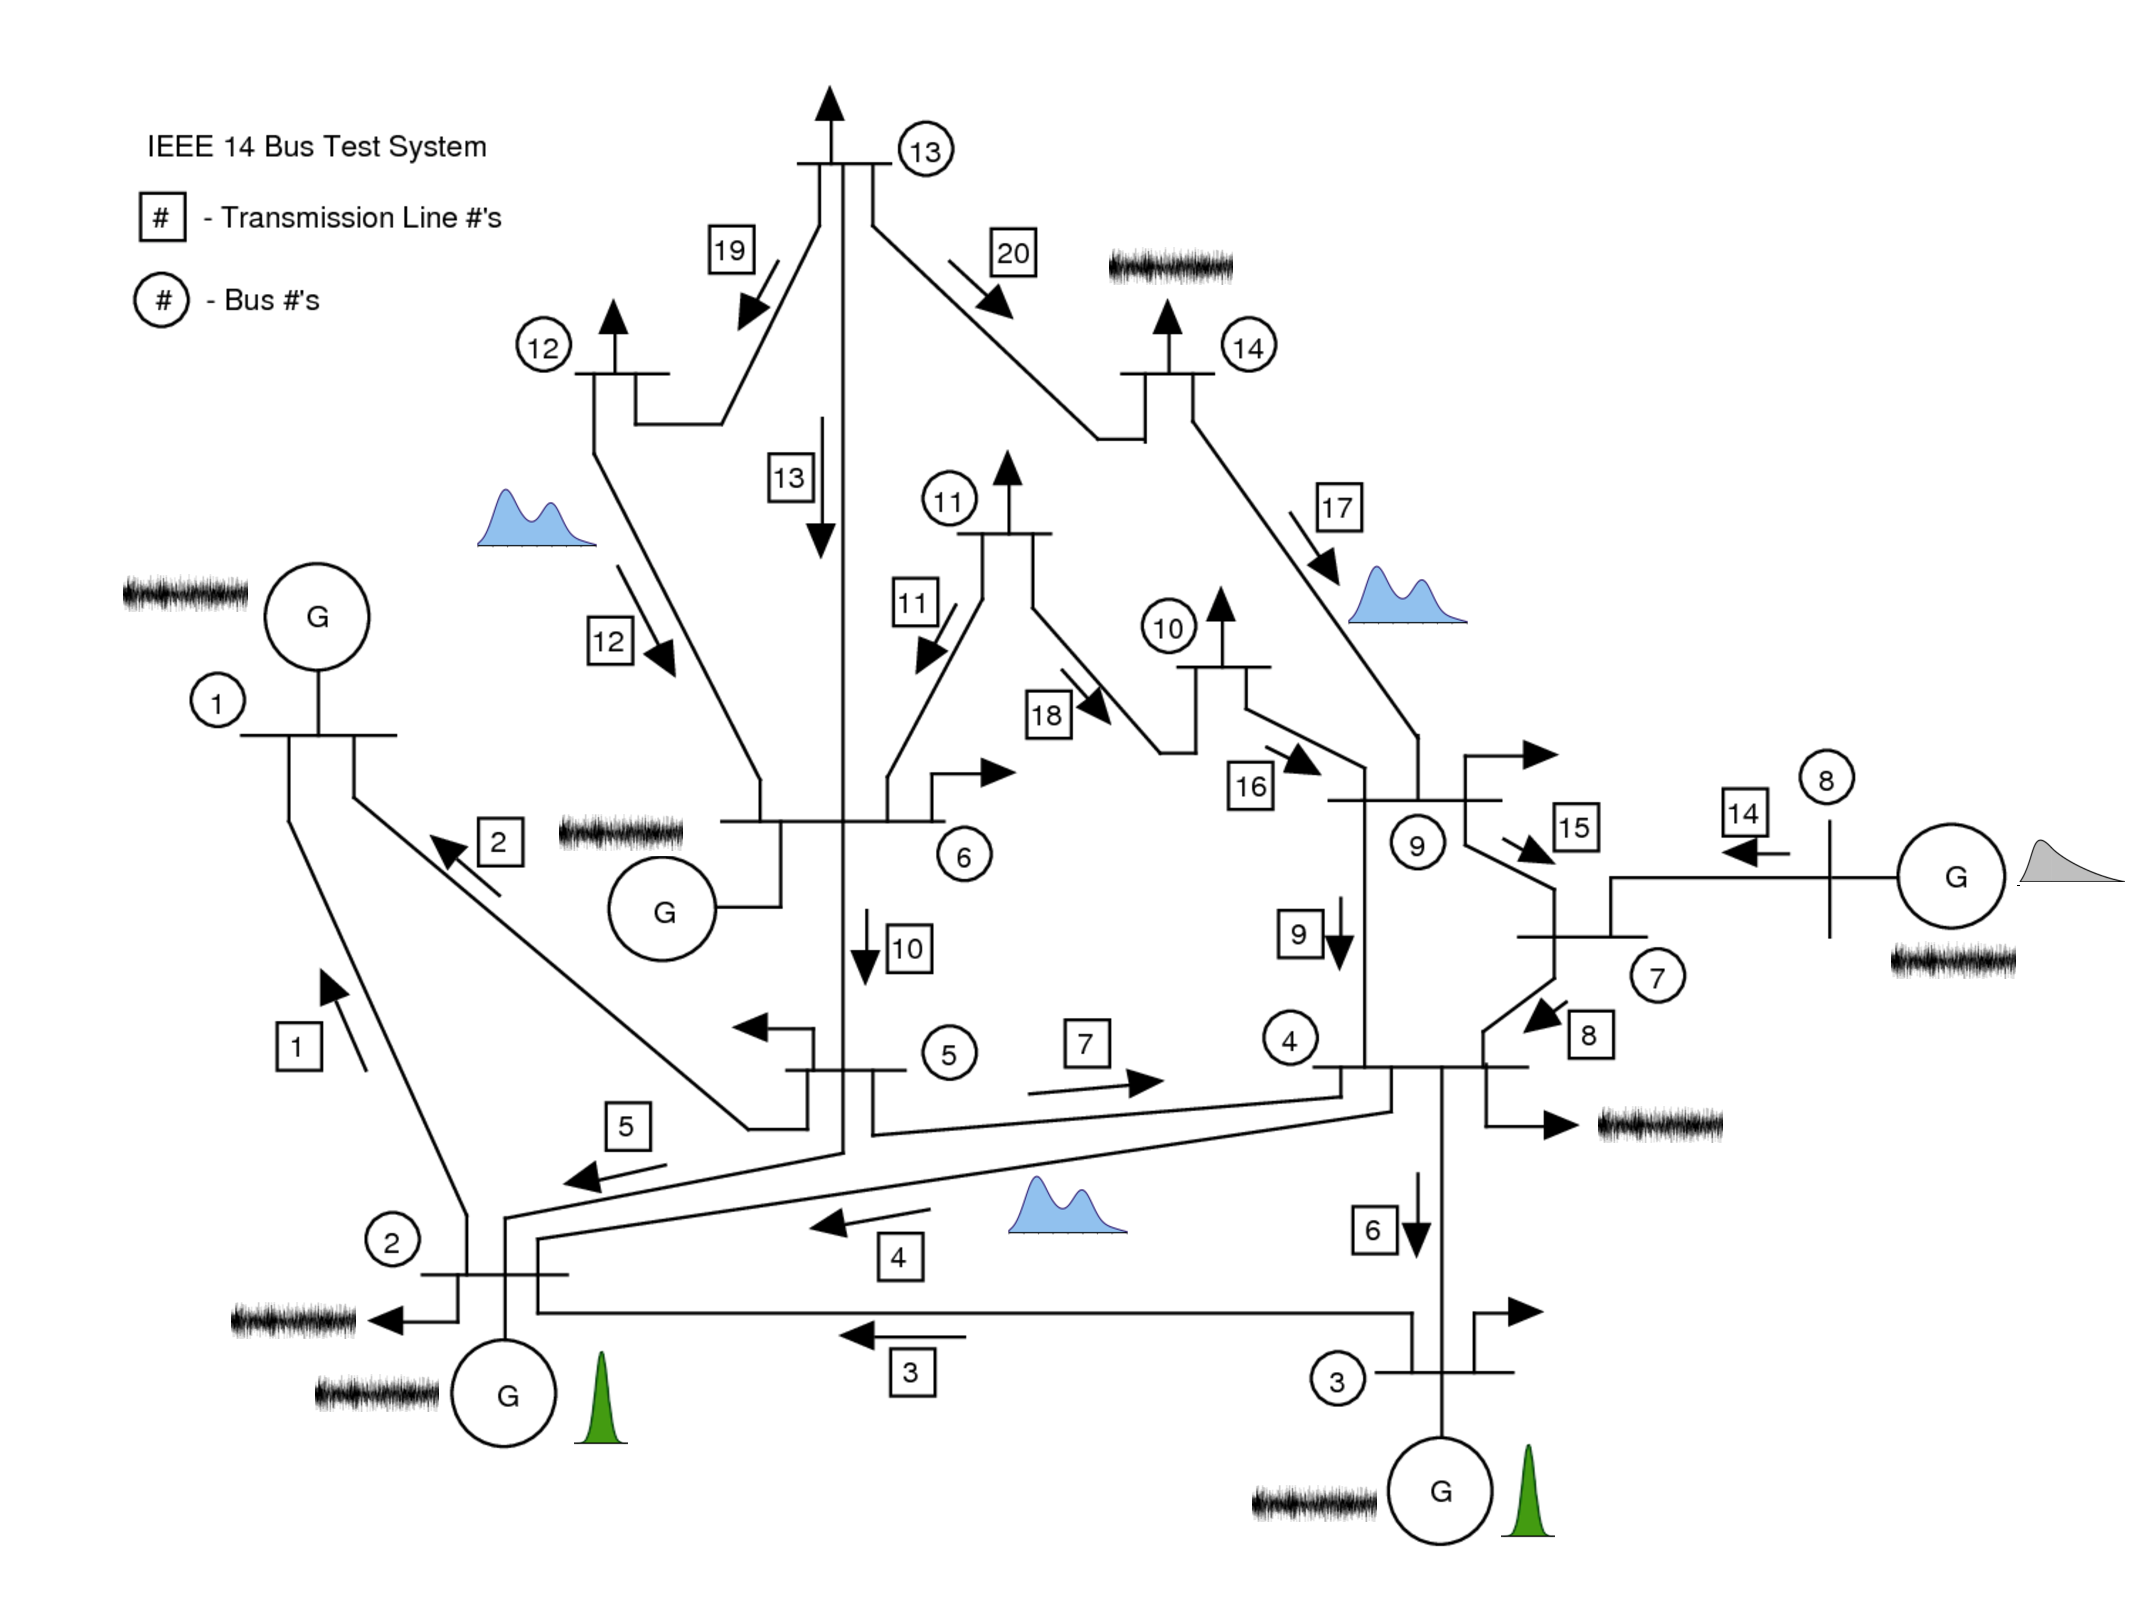
\includegraphics[width=\linewidth]{IEEE14BusWithUnc.pdf}
\caption{\small{A schematic of the IEEE 14 bus test system with stochastic uncertainties. The Uncertainty sources may include stochastic forcing and parametric uncertainties at some generators, random variabilities at some loads, and parametric uncertainties along some transmission lines. For depiction purposes, we indicated the parametric uncertainties as PDFs, and stochastic forcing as intermittent signals.}}
\label{fig:Motivating}
\end{figure}

\begin{figure}
\centering
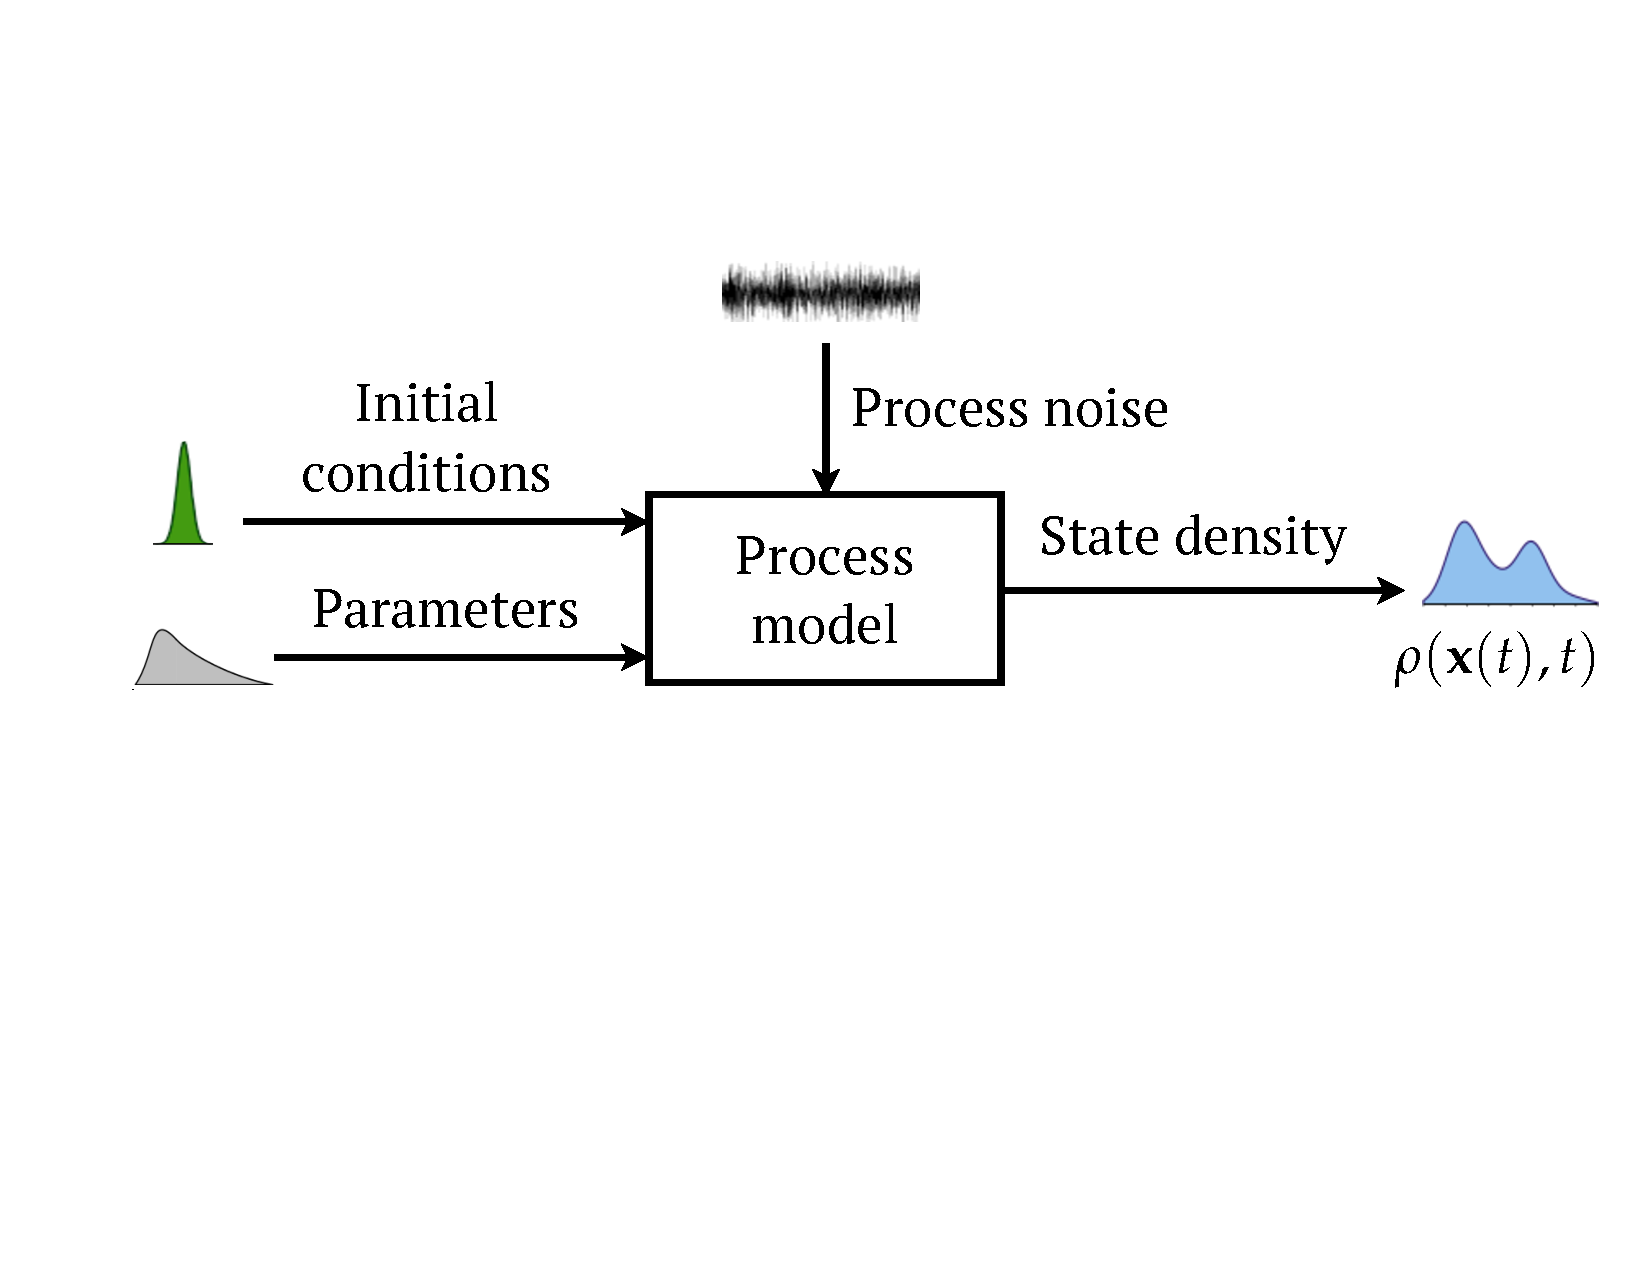
\includegraphics[width=0.9\linewidth]{UncPropBlockDiagm.pdf}
\caption{\small{Block diagram for joint state PDF propagation.}}
\label{fig:UncertaintyPropagation}
\end{figure}

Given a networked power system, one can envisage at least three types of uncertainties affecting the dynamics: initial condition uncertainties in the state variables (e.g., rotor phase angles and angular velocities), parametric uncertainties (e.g., inertia and damping coefficients of the generators, reactance associated with different transmission lines), and stochastic forcing (e.g., intermittencies in renewable power generation, load and ambient temperature fluctuations). Fig. \ref{fig:Motivating} depicts a representative scenario. In addition, one could consider uncertainties due to random change in transmission topology resulting from unexpected outage, and uncertainties due to unmodeled dynamics. Given a statistical description of these uncertainties, our approach is to directly solve the \emph{macroscopic flow} of the joint PDFs governing the probabilistic evolution of the state as summarized in Fig. \ref{fig:UncertaintyPropagation}.


\subsubsection{Related works}
Even though the need for quantifying uncertainties in power systems simulations has been long-recognized \cite{allan8791,allan9296}, early studies were limited to statistical reliability assessment. Dynamic simulations with stochastic uncertainties for purposes such as transient stability analysis have been investigated via \emph{Monte Carlo simulations} \cite{timko1983monte,dong2012numerical,perninge2012importance,odun2012structure}.

 As is well known, the Monte Carlo techniques are easy to apply but the computational cost scales exponentially with the number of dimensions, thus making it prohibitive for realistic power systems dynamic simulation. As an alternative, \emph{probabilistic small signal analysis} \cite{nwankpa1992stochastic,rueda2009assessment,huang2013quasi,dhople2013analysis} have appeared in the power systems literature, albeit at the expense of the additional assumption that the random perturbations remain ``small". \emph{Polynomial chaos and related stochastic collocation methods} \cite{hockenberry2004evaluation,xu2019propagating} can do away with the ``small stochastic perturbation" assumption but due to the finite-dimensional approximation of the probability space, computational performance degrades if the long-term statistics are desired. Furthermore, to cope with the stochasticity, these techniques require simulating a higher-dimensional system than the dimension of the physical state space, which further limits the scalability for nonlinear simulation. More recently, approximation methods such as \emph{stochastic averaging} \cite{ju2018analytical,ju2018stochastic} based on certain energy function \cite{pai1989energy,chang1995direct,sauerpai1998} have appeared. In \cite{maldonado2018uncertainty}, an algorithm for \emph{propagating first few statistical moments} was proposed. However, this leads to moment closure problems since the dimensions of the time-varying sufficient statistics associated with the corresponding transient joint state PDFs are not known in general. 

In a different vein, \emph{deterministic bounded uncertainty models} for power flow simulations have been used \cite{dimitrovski2004boundary,hiskens2006sensitivity,chen2012method,althoff2014formal} for set-valued analysis. These, however, require approximating the underlying nonlinear differential algebraic equations (DAEs) appearing in power system dynamic simulation, and thus lead to conservative analysis. For example, the method in \cite{althoff2014formal} requires converting the nonlinear DAEs to linear DAEs in such a way that guarantees set-valued over-approximation of the reachable sets. Likewise, the convex optimization-based bounded uncertainty propagation methods in \cite{choi2017propagating,choi2018propagating} require second order approximation of the power flow state variables as function of the uncertainties.

\subsubsection{Technical challenges}\label{subsubsec:technicalchallenges}
Several technical challenges need to be overcome to achieve scalable computation enabling the prediction of the joint PDFs over a time horizon of interest. \emph{First}, the trajectory level dynamic models for power systems are inherently nonlinear, which do not preserve Gaussianity, thereby requiring nonparametric prediction of the joint PDFs. \emph{Second}, the joint PDFs for realistic power systems dynamic simulation must evolve over a high dimensional state space, i.e., the joint PDF at any given time has high dimensional support. This necessitates spatial discretization-free algorithms since standard function approximation or interpolation approaches would, in general, be met with ``curse-of-dimensionality" \cite{bellman1957}. The numerical challenges aside, one cannot theoretically guarantee to find a suite of basis functions for the manifold of nonparametric PDFs. \emph{Third}, prediction based on first few statistical moments is challenging since it is not possible to \emph{a priori} guarantee a fixed or even finite dimensional sufficient statistic. For instance, propagating only the mean and covariance could be misleading when the underlying joint PDFs are multi-modal.

\subsubsection{Contributions of this paper}
Our contributions are twofold. {\red{TBD}} 

Our technical approach juxtaposes with the existing literature discussed above, in that we approximate neither the dynamical nonlinearity nor the statistics. Instead of treating the exact nonlinearity as bane, we exploit the geometry induced by the power system's dynamical nonlinearity over the manifold of time-varying joint state PDFs, thereby enabling a new proximal algorithm to compute the transient joint PDFs.

\subsubsection{Notation and organization}
We use boldfaced small letters for vectors, and boldfaced capital letters for matrices. The set of natural numbers is denoted as $\mathbb{N}$. The symbol $\nabla_{\bm{x}}$ denotes the Euclidean gradient operator with respect to (w.r.t.) the vector $\bm{x}$. Thus, $\nabla_{\bm{x}}\cdot$ stands for the divergence, and $\Delta_{\bm{x}}$ stands for the Laplacian w.r.t. vector $\bm{x}$. We use $\langle\cdot,\cdot\rangle$ to denote the standard Euclidean inner product. The real and imaginary parts of a complex number $z$ are denoted via $\Re(z)$ and $\Im(z)$, respectively. The symbol $|\cdot|$ denotes the absolute value, $\otimes$ denotes the Kronecker product, $\det(\cdot)$ stands for the determinant, and the subscript $_{\sharp}$ denotes the pushforward of a PDF via a map. The $n\times n$ identity and zero matrices are denoted as $\bm{I}_{n}$ and $\bm{0}_{n\times n}$, respectively.

The rest of this paper is structured as follows. {\red{TBD}}

%%%%%%%%%%%%%%%%%%%%%%%%%%%%%%%%%%%%%%%%%%%%%%%%%%%%%%%%%%%%%%%%%%%%%%%%%%%%%%%%

\section{Models}\label{sec:models}

\subsection{Sample Path Dynamics}\label{subsec:samplepathdynamics}
We consider the coupled stochastic differential equations (SDEs) associated with the networked-reduced power systems model \cite[Ch. 7]{sauerpai1998}. Specifically, for a power network with $n$ generators, the stochastic dynamics for the $i$-th generator is given by the It\^{o} SDEs
\begin{subequations}
\begin{align}
&{\mathrm{d}}\theta_{i} = \omega_{i}\:{\mathrm{d}}t,\label{RotAngleGen}\\
&m_{i}\:{\mathrm{d}}\omega_{i} =	\left(\!P_{i} - \gamma_{i}\omega_{i} - \displaystyle\sum_{j=1}^{n} k_{ij}\sin\left(\theta_{i}-\theta_{j}-\varphi_{ij}\right)\!\right){\mathrm{d}}t \nonumber\\
&\qquad\qquad\qquad\qquad\qquad\qquad\qquad\qquad\qquad+\sigma_{i}\:{\mathrm{d}}w_{i},
\end{align}
\label{ItoSDEcomponentlevel}
\end{subequations}
where the state variables are the rotor angles $\theta_{i}\in[0,2\pi)$ and the rotor angular velocities $\omega_{i}\in\mathbb{R}$, for $i\in\{1,\hdots,n\}$. The stochastic forcing is modeled through the standard Wiener process $w_{i}(t)$, and the diffusion coefficient $\sigma_{i}>0$ denotes the intensity of stochastic forcing at the $i$-th generator. 

With the $i$-th generator, we associate its inertia $m_{i}>0$ and damping coefficient $\gamma_{i}>0$. The other parameters: the \emph{effective power input} $P_{i}$, the \emph{phase shift} $\varphi_{ij}\in[0,\frac{\pi}{2})$, and the \emph{coupling coefficients} $k_{ij}\geq 0$, depend on the network reduced admittance matrix $\bm{Y}\equiv[Y_{ij}]_{i,j=1}^{n}\in\mathbb{C}^{n\times n}$. Specifically,
\begin{subequations}
\begin{align}
 P_{i} &= P_{i}^{\text{mech}} - E_{i}^{2} \Re\left(Y_{ii}\right), \\
 \varphi_{ij} &= \begin{cases} -\arctan\left(\dfrac{\Re\left(Y_{ij}\right)}{\Im\left(Y_{ij}\right)}\right), & \text{if}\;i\neq j,\\
 0, & \text{otherwise},
 \end{cases}\\
 k_{ij} &= \begin{cases} E_{i}E_{j} \vert Y_{ij}\vert, & \text{if}\;i\neq j,\\
 0, & \text{otherwise},
 \end{cases}
\end{align}
\end{subequations}
where $P_{i}^{\text{mech}}$ is the mechanical power input, and $E_{i}$ is the internal voltage (magnitude) for generator $i$.

% The coupling coefficients $k_{ij}$, roughly speaking, denote the maximum power transferred between generators $i$ and $j$ with $k_{ii}=0$ for $i\in\{1,\hdots,n\}$. In general, $k_{ij}$ is a function of the internal voltages at the $i$-th and $j$-th generator, and the magnitude of the $(i,j)$-th entry of the network reduced admittance matrix. We suppose that the elements $k_{ij}$ comprise a coupling matrix $\bm{K}$ of appropriate dimension. 

One can view (\ref{ItoSDEcomponentlevel}) as the noisy version of the second order nonuniform Kuramoto oscillator model \cite{dorfler2012synchronization,rodrigues2016kuramoto}, also known as the structure preserving power network model \cite{odun2012structure}, given by
\begin{align}
m_{i}\ddot{\theta}_{i} + \gamma_{i}\dot{\theta}_{i} &= P_{i} - \displaystyle\sum_{j=1}^{n} k_{ij}\sin\left(\theta_{i} - \theta_{j} - \varphi_{ij}\right) \nonumber\\
&\qquad\qquad+ \sigma_{i} \times \text{stochastic forcing},
\label{LangevinForm}	
\end{align}
where the stochastic forcing is standard Gaussian white noise. 

We define the \emph{positive diagonal} matrices
\begin{align*}
\bm{M} &:= {\rm{diag}}\left(m_{1},\hdots,m_{n}\right), \nonumber\\
\bm{\Gamma} &:= {\rm{diag}}\left(\gamma_{1},\hdots,\gamma_{n}\right),\nonumber\\
\bm{\Sigma} &:= {\rm{diag}}\left(\sigma_{1},\hdots,\sigma_{n}\right),
%\label{PosDiagMatrices}	
\end{align*}
and rewrite (\ref{ItoSDEcomponentlevel}) as a mixed conservative-dissipative SDE in state vector $\bm{x} := (\bm{\theta},\bm{\omega})^{\top} \in \mathbb{T}^{n} \times \mathbb{R}^{n}$ as
\begin{align}
\begin{pmatrix}
{\mathrm{d}}\bm{\theta}\\
{\mathrm{d}}\bm{\omega}	
\end{pmatrix}
\! = \!\begin{pmatrix}
\bm{\omega}\\
-\bm{M}^{-1}\nabla_{\bm{\theta}}V(\bm{\theta}) -\bm{M}^{-1}\bm{\Gamma}\bm{\omega}  	
\end{pmatrix}{\mathrm{d}}t + \!\begin{pmatrix}
 \bm{0}_{n\times n}\\
 \bm{M}^{-1}\bm{\Sigma}	
 \end{pmatrix}{\mathrm{d}}\bm{w},
\label{ItoSDEvectorlevel}
\end{align}
where 
%$\odot$ denotes element-wise product, $\oslash$ denotes element-wise division, the , the rotor inertia vector $\bm{m} = (m_{1},\hdots,m_{n})^{\top}\in\mathbb{R}^{n}_{>0}$, the rotor damping coefficient vector $\bm{\gamma} = (\gamma_{1}, \hdots, \gamma_{n})^{\top}\in\mathbb{R}^{n}_{>0}$, the diffusion coefficient vector $\bm{\sigma} = (\sigma_{1}, \hdots, \sigma_{n})^{\top}\in\mathbb{R}^{n}_{>0}$, and 
$\bm{w}\in\mathbb{R}^{n}$ is the standard vector Wiener process, $\mathbb{T}^{n}$ denotes the $n$-torus $[0,2\pi)^{n}$, and the potential function $V : \mathbb{T}^{n} \mapsto \mathbb{R}$ is given by
\begin{align}
V(\bm{\theta}) := \displaystyle\sum_{i=1}^{n} P_{i}\theta_{i} + \!\displaystyle\sum_{(i,j)\in\mathcal{E}}\!k_{ij}\left(1 - \cos(\theta_{i}-\theta_{j}-\varphi_{ij})\right),
\label{potential}	
\end{align}
wherein $\mathcal{E}$ is the set of edges for the underlying graph modeling the power system network. The potential (\ref{potential}) has a natural energy function interpretation and can also be motivated by a mechanical mass-spring-damper analogy \cite{dorfler2013synchronization,ishizaki2018}. The function $V$ is continuously differentiable, bounded below, and goes to $+\infty$ as $\|\bm{\theta}\|_{2}\rightarrow +\infty$.
%In the development below, an important role will be played by the ``Hamiltonian-like" function
%\begin{align}
%H(\bm{x})\equiv H(\bm{\theta},\bm{\omega}) := \frac{1}{2}\bm{\omega}^{\top}{\rm{diag}}\left(\bm{\gamma}\oslash\bm{m}\right)\bm{\omega} \: + \: V(\bm{\theta}).
%\label{hamiltonian}	
%\end{align}


\subsection{Macroscopic Dynamics}\label{subsec:macroscopic}
Given the sample path dynamics \eqref{ItoSDEcomponentlevel} or equivalently \eqref{ItoSDEvectorlevel}, a prescribed initial joint state PDF 
\begin{align}
\rho_{0}(\bm{x})\equiv\rho(t=t_{0},\bm{\theta}(t_{0}),\bm{\omega}(t_{0}))
\label{FPKInitCond}	
\end{align} 
denoting initial condition uncertainties at time $t=t_{0}$, and prescribed parametric uncertainties given by the joint parameter PDF $\rho_{\text{param}}$, the uncertainty propagation problem calls for computing the transient joint state PDFs $\rho(t,\bm{x})\equiv\rho(t,\bm{\theta},\bm{\omega})$ for any desired time $t \geq t_{0}$, which is a nonnegative function supported on the state space $\mathbb{T}^{n} \times \mathbb{R}^{n}$ satisfying $\int \rho = 1$ for all $t\geq t_{0}$.

The corresponding macroscopic dynamics governing the flow of the joint state PDF $\rho(t,\bm{\theta},\bm{\omega})$ is given by a kinetic Fokker-Planck partial differential equation (PDE)
\begin{align}
\frac{\partial \rho}{\partial t} &= - \langle \bm{\omega},\nabla_{\bm{\theta}}\rho \rangle  + \nabla_{\bm{\omega}} \cdot \left( \rho \left( \bm{M}^{-1}\bm{\Gamma}\bm{\omega} + \bm{M}^{-1}\nabla_{\bm{\theta}}V(\bm{\theta}) \right.\right.\nonumber\\
&\qquad\qquad\qquad \left.\left. +\frac{1}{2} \bm{M}^{-1}\bm{\Sigma}\bm{\Sigma}^{\top}\bm{M}^{-1} \nabla_{\bm{\omega}} \log \rho \right) \right),
\label{KineticFPK}	
\end{align}
subject to the initial condition \eqref{FPKInitCond} and the joint parameter PDF $\rho_{\text{param}}$. A direct numerical solution of this PDE initial value problem using conventional discretization (e.g., finite difference) or function approximation techniques will not be scalable in general, as explained in Sec. \ref{subsubsec:technicalchallenges}. In the next Section, we discuss how a measure-valued variational recursion proposed in our recent works \cite{caluya2019ACC,caluya2019TAC,halder2020hopfield,caluya2021TAC} can be employed to address this challenge.

We mention here that (\ref{ItoSDEvectorlevel}) has been used in \cite{ju2018analytical,ju2018stochastic} for uncertainty propagation via stochastic averaging approximation where the univariate energy PDF was proposed as a ``proxy" for the entire joint PDF. Most relevant to our approach in the power systems literature is the work in \cite{wang2013fokker}, which indeed voiced the need for computing the transient joint PDFs but only dealt with the single-machine-infinite-bus case -- simplest instance of (\ref{ItoSDEvectorlevel}). The resulting bivariate Fokker-Planck PDE in \cite{wang2013fokker} was solved via finite element discretization, and revealed rich stochastic dynamics and nontrivial transient stability aspects even in this simple case. However, it is unreasonable to expect that a finite element discretization, or in fact any spatial discretization scheme to solve (\ref{KineticFPK}) for moderately large $n$ in {\red{minutes}} of computational time, thereby limiting our current ability for realistic power systems simulation with stochastic variability. This calls for fundamentally re-thinking what does it mean to solve the PDE (\ref{KineticFPK}) for dynamics (\ref{ItoSDEvectorlevel}).

%%%%%%%%%%%%%%%%%%%%%%%%%%%%%%%%%%%%%%%%%%%%%%%%%%%%%%%%%%%%%%%%%%%%%%%%%%%%%%%%

\section{Measure-valued Proximal Recursion}\label{sec:prox}
\subsection{Generalized Gradient Descent}\label{subsec:GenGradDescent}
Let $\mathcal{P}_{2}\left(\mathbb{T}^{n} \times \mathbb{R}^{n}\right)$ denote the manifold of all joint PDFs supported over the state space $\mathbb{T}^{n} \times \mathbb{R}^{n}$, with finite second raw moments. Symbolically,
\begin{align}
\mathcal{P}_{2}\left(\mathbb{T}^{n} \times \mathbb{R}^{n}\right) := &\bigg\{\rho : \mathbb{T}^{n} \times \mathbb{R}^{n} \mapsto \mathbb{R}_{\geq 0} \mid \int \rho = 1,\nonumber\\
&\hspace*{-0.8in}\int\bm{x}^{\top}\bm{x}\:\rho(\bm{x})\:\differential\bm{x} <\infty\; \text{for all}\;\bm{x}\equiv(\bm{\theta},\bm{\omega})^{\top}\in\mathbb{T}^{n} \times \mathbb{R}^{n} \bigg\}.
\label{DefP2}	
\end{align}
We propose to solve the initial value problem for the PDE \eqref{KineticFPK} by viewing its flow $\rho(t,\bm{\theta},\bm{\omega})$ as the gradient descent of some functional $\Phi:\mathcal{P}_{2}\left(\mathbb{T}^{n} \times \mathbb{R}^{n}\right)\mapsto \mathbb{R}_{\geq 0}$ w.r.t. some distance 
\[{\rm{dist}}:\mathcal{P}_{2}\left(\mathbb{T}^{n} \times \mathbb{R}^{n}\right)\times\mathcal{P}_{2}\left(\mathbb{T}^{n} \times \mathbb{R}^{n}\right)\mapsto\mathbb{R}_{\geq 0}.\]
We now explain this idea in detail.

For $k\in\mathbb{N}$, and for some chosen step size $h>0$, we discretize time as $t_{k} := kh$, and define the infinite dimensional proximal operator of the functional $h\Phi$ w.r.t. the distance ${\rm{dist}}(\cdot,\cdot)$, given by
\begin{eqnarray}
{\text{prox}}^{{\rm{dist}}}_{h\Phi}(\varrho_{k-1}) := \underset{\varrho\in\mathcal{P}_{2}} {{\rm{arg\:inf}}}\: \frac{1}{2} {\rm{dist}}^{2}\left(\varrho,\varrho_{k-1}\right) + h\: \Phi(\varrho).
\label{InfiniteDimProxOpDef}
\end{eqnarray}
Now consider a proximal recursion over the manifold $\mathcal{P}_{2}$ as
\begin{eqnarray}
\varrho_{k} = {\text{prox}}^{{\rm{dist}}}_{h\Phi}(\varrho_{k-1}), \quad k\in\mathbb{N}, \quad \varrho_{0}(\bm{x}) := \rho_{0}(\bm{x}).
\label{ProxRecursionInfiniteDim}	
\end{eqnarray}
Given the PDE \eqref{KineticFPK}, we would like to design the functional pair $\left(\Phi,{\rm{dist}}\right)$ such that the sequence of functions $\{\varrho_{k}\}_{k\in\mathbb{N}}$ generated by the proximal recursion \eqref{ProxRecursionInfiniteDim}, in the small time step limit, converges to the flow $\rho(t=kh,\bm{\theta},\bm{\omega})$ generated by the PDE initial value problem of interest. In particular,
\begin{align}
\varrho_{k}(\bm{\theta},\bm{\omega}) \xrightarrow{h\downarrow 0} \rho(t=kh,\bm{\theta},\bm{\omega}) \;\text{in}\;L^{1}\left(\mathbb{T}^{n} \times \mathbb{R}^{n}\right).
\label{ConvergenceGuarantee}	
\end{align}
We remark here that \eqref{DefP2}, \eqref{InfiniteDimProxOpDef}, \eqref{ProxRecursionInfiniteDim}, \eqref{ConvergenceGuarantee} can be written more generally in therms of the joint probability measures instead of PDFs, i.e., even when the underlying measures are not absolutely continuous.

Notice that the proximal recursions given by \eqref{InfiniteDimProxOpDef}-\eqref{ProxRecursionInfiniteDim} define an infinite dimensional gradient descent of the functional $h\Phi$ over $\mathcal{P}_{2}$ w.r.t. the distance ${\rm{dist}}$. This is reminiscent of the finite dimensional gradient descent, where a gradient flow generated by an ordinary differential equation initial value problem can be recovered as the small time step limit of the sequence of vectors generated by a standard Euclidean proximal recursion; see e.g., \cite[Sec. I]{caluya2019TAC}.

That the flow generated by a Fokker-Planck PDE initial value problem can be recovered from a variational recursion of the form \eqref{ProxRecursionInfiniteDim} was first proposed in \cite{jordan1998variational}, showing that when the drift in the sample path dynamics is a gradient vector field and the diffusion is a scalar multiple of identity matrix, then ${\rm{dist}}(\cdot,\cdot)$ can be taken as the Wasserstein-2 metric arising in the theory of optimal transport \cite{villani2003topics} with $\Phi(\cdot)$ as the free energy functional. In particular, the functional $\Phi$ serves as a Lyapunov functional in the sense $\frac{\differential}{\differential t}\Phi < 0$ along the transient solution of the Fokker-Planck PDE initial value problem. This idea has since been generalized to many other types of PDE initial value problems, see e.g., \cite{ambrosio2008gradient,santambrogio2017euclidean}. 

The algorithmic appeal of the proximal recursion \eqref{ProxRecursionInfiniteDim} is that it opens up the possibility to compute the solution of the PDE initial value problem via recursive convex minimization. A point cloud-based proximal algorithm was proposed in \cite{caluya2019ACC,caluya2019TAC} which was reported to have very fast runtime. Notice that even though the drift in \eqref{ItoSDEvectorlevel} is \emph{not} a gradient vector field, the algorithm in \cite[Sec. V.B]{caluya2019TAC} constructed a pair $\left(\Phi,{\rm{dist}}\right)$ such that \eqref{ProxRecursionInfiniteDim} provably approximates the transient solution of the corresponding kinetic Fokker-Planck PDE with guarantee \eqref{ConvergenceGuarantee}. However, that algorithm cannot be applied to \eqref{KineticFPK} as is. The reasons are explained next.

\subsection{Statistical Mechanics Perspective}
A new difficulty for our SDE \eqref{ItoSDEvectorlevel} is that we have \emph{anisotropic} degenerate diffusion, i.e., the strengths of the noise acting in the last $n$ components of \eqref{ItoSDEvectorlevel} are nonuniform since $\bm{M}^{-1}\bm{\Sigma}$ is not identity. This complicates the matter because the construction of the functional $\Phi$ in \eqref{ProxRecursionInfiniteDim} is usually motivated via free energy considerations utilizing the structure of the \emph{stationary} PDF $\rho_{\infty}(\bm{\theta},\bm{\omega})$ for \eqref{KineticFPK}. The $\rho_{\infty}$ is, in turn, guaranteed to be a unique \emph{Boltzmann distribution} of the form\footnote{here $Z$ is a normalizing constant known as the ``partition function".}
\begin{subequations}
\begin{align}
\rho_{\infty}\left(\bm{\theta},\bm{\omega}\right) &= \dfrac{1}{Z}\exp\left(-\beta H\right), \\
H(\bm{\theta},\bm{\omega}) &:= V(\bm{\theta}) + \frac{1}{2}\langle\bm{\omega},\bm{M\omega}\rangle,	
\end{align}	
\label{BoltzmannPDF}
\end{subequations}
\emph{if and only if} the so-called \emph{Einstein relation} \cite{hernandez1989equilibrium,chen2015fast} holds:
\begin{align}
\bm{\Sigma}\bm{\Sigma}^{\top} = \beta^{-1}\left(\bm{\Gamma} + \bm{\Gamma}^{\top}\right) \quad\text{for some}\;\beta > 0.
\label{EinsteinRelation}	
\end{align}
In our case, $\bm{\Sigma,\Gamma}$ are positive diagonal, and \eqref{EinsteinRelation} is equivalent to $\sigma_{i}^{2} \propto \gamma_{i}$ for all $i=1,\hdots,n$.

In the power systems context, we cannot relate the damping coefficients $\gamma_i$ with the squared intensities of stochastic forcing $\sigma_{i}^{2}$ for the generators. Thus, \eqref{EinsteinRelation} will not hold in practice, meaning either we cannot guarantee existence-uniqueness for $\rho_{\infty}$, or even if $\rho_{\infty}$ exists, it will not be of the form \eqref{BoltzmannPDF}. On one hand, this implies that our construction of $\Phi$ may not be guided by free energy considerations. On the other hand, since we are only interested in computing the transient joint PDFs, i.e., \emph{non-equilibrium} statistical mechanics, the lack of a fluctuation-dissipation relation like \eqref{EinsteinRelation} should not be a fundamental impediment in setting up a recursion such as \eqref{ProxRecursionInfiniteDim}. We next show that a simple change of variable can indeed circumvent this issue. 


\subsection{From Anisotropic to Isotropic Degenerate Diffusion}\label{subsec:FromAnisoToIso}
Consider the $2n\times 2n$ matrix
\begin{align}
\bm{\Psi}:= \bm{I}_{2} \otimes \left(\bm{M}\bm{\Sigma}^{-1}\right), \label{DefPsi}	
\end{align}
and define the invertible linear map
\begin{align}
\begin{pmatrix}
\bm{\theta}\\
\bm{\omega}	
\end{pmatrix} \mapsto \begin{pmatrix}
\bm{\xi}\\
\bm{\eta}	
\end{pmatrix} := \bm{\Psi} \begin{pmatrix}
\bm{\theta}\\
\bm{\omega}	
\end{pmatrix}. \label{ChangeOfVar}
\end{align}
Applying It\^{o}'s lemma \cite[Ch. 4.2]{oksendal2013stochastic} to the map \eqref{ChangeOfVar}, and using \eqref{ItoSDEvectorlevel}, we find that the transformed state vector $(\bm{\xi},\bm{\eta})^{\top}$ solves the It\^{o} SDE 
\begin{align}
\begin{pmatrix}
{\mathrm{d}}\bm{\xi}\\
{\mathrm{d}}\bm{\eta}	
\end{pmatrix}
\! = \!\begin{pmatrix}
\bm{\eta}\\
-\nabla_{\bm{\xi}}U(\bm{\xi}) -\nabla_{\bm{\eta}}F\left(\bm{\eta}\right)  	
\end{pmatrix}{\mathrm{d}}t + \!\begin{pmatrix}
 \bm{0}_{n\times n}\\
 \bm{I}_{n}	
 \end{pmatrix}{\mathrm{d}}\bm{w},
\label{XiEtaVectorSDE}	
\end{align}
where the potentials
{\small{\begin{subequations}
\begin{align}
U(\bm{\xi}) &:= \!\displaystyle\sum_{i=1}^{n}\!\frac{1}{\sigma_{i}}P_{i}\xi_{i} + \!\!\!\! \displaystyle\sum_{(i,j)\in\mathcal{E}}\!\!\dfrac{m_{i}}{\sigma_{i}^{2}}k_{ij}\!\left(\!1 \!- \!\cos\!\left(\!\dfrac{\sigma_{i}}{m_{i}}\xi_{i} + \dfrac{\sigma_{j}}{m_{j}}\xi_{j} - \varphi_{ij}\!\!\right)\!\right), \label{defU}\\
F(\bm{\eta}) &:= \dfrac{1}{2}\langle\bm{\eta},\bm{M}^{-1}\bm{\Gamma}\bm{\eta}\rangle. \label{defF}	
\end{align}
\label{NewPotentials}	
\end{subequations}}}


Notice that \eqref{XiEtaVectorSDE} is a mixed conservative-dissipative SDE with \emph{isotropic} degenerate diffusion. In particular, the pushforward of the known initial joint PDF \eqref{FPKInitCond} via $\bm{\Psi}$, is given by
\begin{align}
\tilde{\rho}_{0}(\bm{\xi},\bm{\eta}) := \bm{\Psi}_{\sharp} \rho_{0} 
&= \dfrac{\rho_{0}\left(\bm{\Psi}^{-1} \begin{pmatrix}
\bm{\xi}\\
\bm{\eta}	
\end{pmatrix}\right)}{|\det\left(\bm{\Psi}\right)|} \nonumber\\
&= \dfrac{\rho_{0}\left(\bm{\Sigma}\bm{M}^{-1}\bm{\xi},\bm{\Sigma}\bm{M}^{-1}\bm{\eta}\right)}{\left(\displaystyle\prod_{i=1}^{n}m_{i}/\sigma_{i}\right)^{\!2}},
\label{PushforwardOfIC}	
\end{align}
where we used the standard properties of the Kronecker product. The transient joint state PDF $\tilde{\rho}(t,\bm{\xi},\bm{\eta})$ corresponding to \eqref{XiEtaVectorSDE} solves the PDE initial value problem
\begin{subequations}
\begin{align}
&\dfrac{\partial\tilde{\rho}}{\partial t} = -\langle\bm{\eta},\nabla_{\bm{\xi}}\tilde{\rho}\rangle + \nabla_{\bm{\eta}}\cdot\left(\tilde{\rho}\left(\nabla_{\bm{
\xi}}U(\bm{\xi})+\nabla_{\bm{\eta}}F(\bm{\eta})\right)\right) + \dfrac{1}{2}\Delta_{\bm{\eta}}\tilde{\rho}, \label{NewPDE}\\
&\tilde{\rho}(t=t_{0},\bm{\xi},\bm{\eta}) = \underbrace{\tilde{\rho}_{0}(\bm{\xi},\bm{\eta})}_{\text{from}\;\eqref{PushforwardOfIC}}. \label{NewIC}	
\end{align}
\label{TransformedPDEivp}	
\end{subequations}
In other words, \eqref{TransformedPDEivp} is the macroscopic dynamics corresponding to the sample path dynamics \eqref{XiEtaVectorSDE}.

Since \eqref{NewPDE} is a kinetic Fokker-Planck PDE with isotropic degenerate diffusion, our strategy is to perform a proximal recursion of the form \eqref{ProxRecursionInfiniteDim} for \eqref{TransformedPDEivp} in $(\bm{\xi},\bm{\eta})$ coordinates, and then to pushforward the resulting joint PDFs via $\bm{\Psi}^{-1}$ to the original state space. This is what we detail next.


\subsection{Proximal Update}\label{subsec:ProxUpdate}
Looking at \eqref{NewPotentials} and \eqref{NewPDE}, it is natural to consider the energy functional 
\begin{align}
\Phi(\tilde{\rho}) := \displaystyle\int_{\mathbb{T}^{n}\times\mathbb{R}^{n}}\left(U(\bm{\xi})+ \frac{1}{2}\|\bm{\eta}\|_{2}^{2} + \frac{1}{2}\log\tilde{\rho}\right)\tilde{\rho}\:\differential\bm{\xi}\differential\bm{\eta},
\label{LyapButNotProx}	
\end{align}
which is the sum of a potential energy (expected value of $U$), a kinetic energy (expected value of $\frac{1}{2}\|\bm{\eta}\|_{2}^{2}$), and an internal energy (scaled negative entropy, the entropy being $-\int\tilde{\rho}\log\tilde{\rho}$). Indeed, it can be shown that (Appendix \ref{AppLyap}) the functional \eqref{LyapButNotProx} is a Lyapunov functional, i.e., $\frac{\differential}{\differential t}\Phi \leq 0$ along the solution of \eqref{NewPDE}.

However, it is not possible  


%%%%%%%%%%%%%%%%%%%%%%%%%%%%%%%%%%%%%%%%%%%%%%%%%%%%%%%%%%%%%%%%%%%%%%%%%%%%%%%%


\section{Proximal Algorithm}\label{sec:ProxAlgo}

%%%%%%%%%%%%%%%%%%%%%%%%%%%%%%%%%%%%%%%%%%%%%%%%%%%%%%%%%%%%%%%%%%%%%%%%%%%%%%%%

\section{Numerical Simulations}\label{sec:NumericalSimulations}

%%%%%%%%%%%%%%%%%%%%%%%%%%%%%%%%%%%%%%%%%%%%%%%%%%%%%%%%%%%%%%%%%%%%%%%%%%%%%%%%


\section{Conclusion}\label{sec:conclusion}
The conclusion goes here.


\appendices
\section{Showing $\frac{\differential}{\differential t}\Phi(\tilde{\rho})$ along \eqref{NewPDE}}\label{AppLyap}
The ma











\begin{figure}
\centering
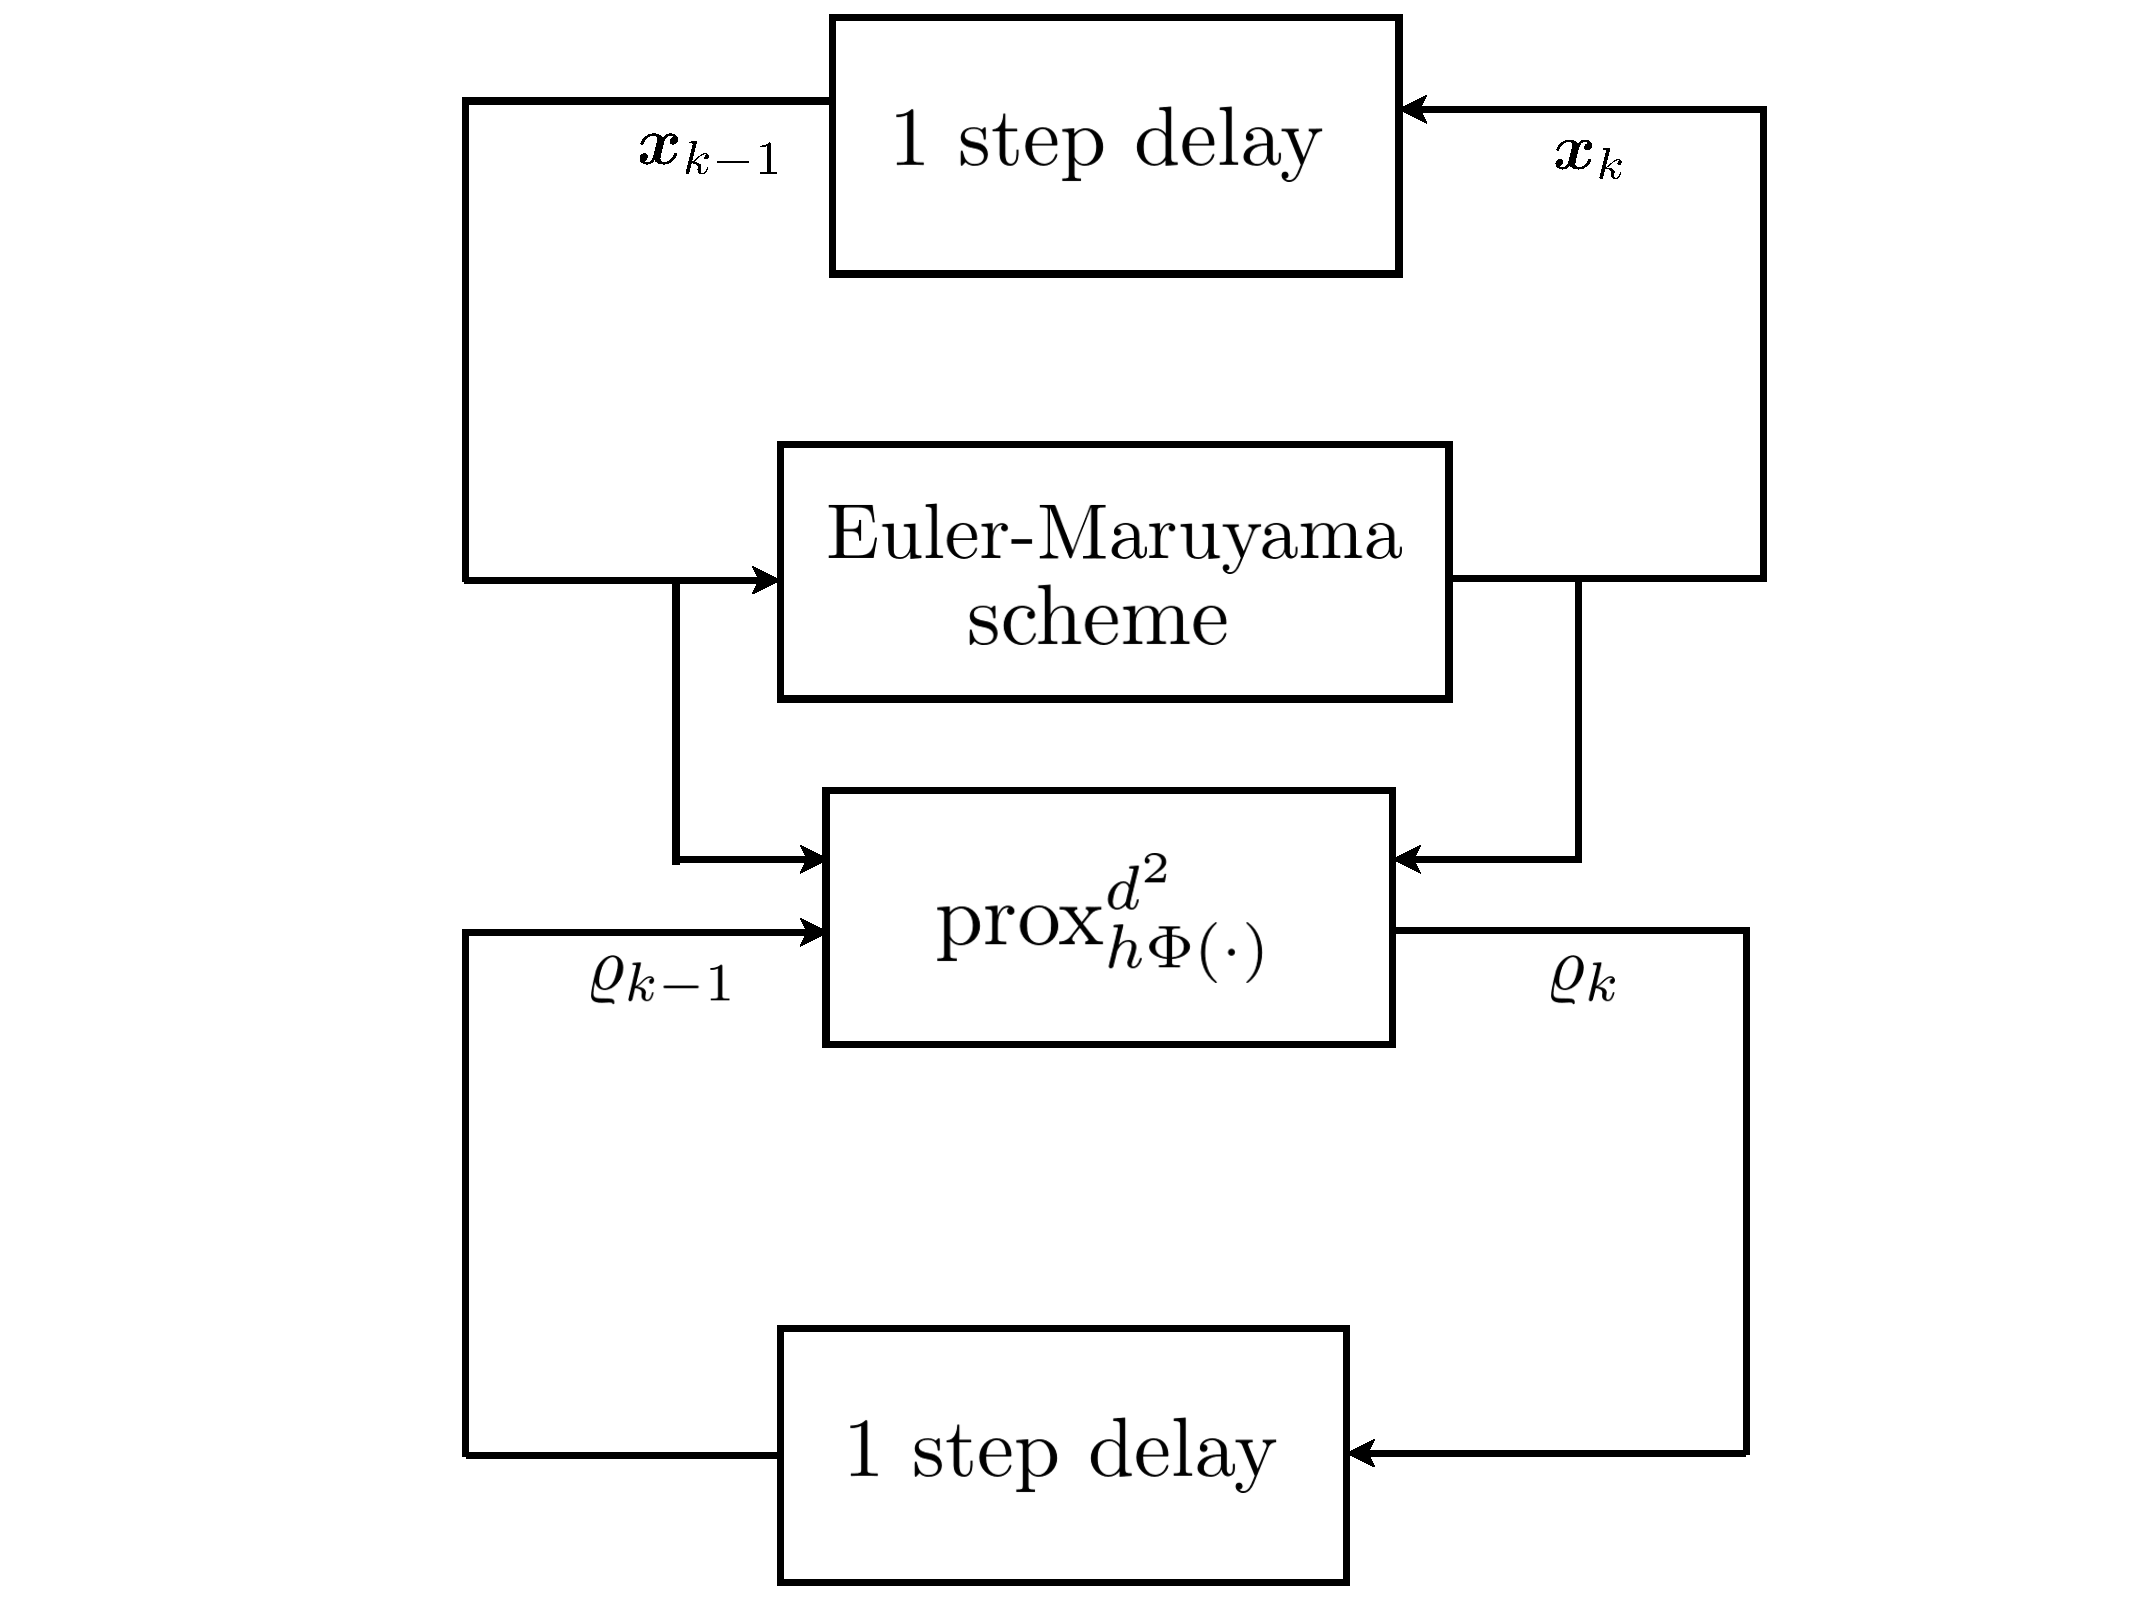
\includegraphics[width=.8\linewidth]{BlockDiagm.pdf}
\caption{\small{Schematic of the proposed algorithmic setup for propagating the joint state PDF as probability weighted scattered point cloud $\{\bm{x}_{k}^{i},\varrho_{k}^{i}\}_{i=1}^{N}$. The location of the points $\{\bm{x}_{k}^{i}\}_{i=1}^{N}$ can be updated by Euler-Maruyama scheme applied to (\ref{ItoSDEvectorlevel}); the corresponding probability weights $\{\varrho_{k}^{i}\}_{i=1}^{N}$ can be updated via discrete version of the proximal recursion (\ref{ProxRecursionInfiniteDim}).}}
\label{fig:BlockDiagm}
\end{figure}



%%%%%%%%%%%%%%%%%%%%%%%%%%%%%%%%%%%%%%%%%%%%%%%%%%%%%%%%%%%%%%%%%%%%%%%%%%%%%%%%

\begin{thebibliography}{99}

\bibitem{schwalbe2015mathematical}
M. Schwalbe, \emph{Mathematical Sciences Research Challenges for the Next-generation Electric Grid: Summary of a Workshop}, National Academies Press, 2015. 

% lit review starts here
%========================
\bibitem{allan8791}
R.N. Allan, R. Billinton, A.M. Breipohl, and C.H. Grigg, ``Bibliography On the Application of Probability Methods in Power Systems Reliability Evaluation 1987--1991", \emph{IEEE Transactions on Power Systems}, Vol. 9, pp. 41--49, 1994. 

\bibitem{allan9296}
------, ``Bibliography On the Application of Probability Methods in Power Systems Reliability Evaluation 1992--1996", \emph{IEEE Transactions on Power Systems}, Vol. 14, pp. 51--57, 1999.

%==== MC =====

\bibitem{timko1983monte}
K.J. Timko, A. Bose, and P.M. Anderson, ``Monte Carlo Simulation of Power System Stability", 
\emph{IEEE Transactions on Power Apparatus and Systems}, Vol. PAS-102, No. 10, pp. 3453--3459, 1983.

\bibitem{dong2012numerical}
Z.Y. Dong, J.H. Zhao, and D.J. Hill, ``Numerical Simulation for Stochastic Transient Stability Assessment", \emph{IEEE Transactions on Power Systems}, Vol. 27, No. 4, pp. 1741--1749, 2012. 

\bibitem{perninge2012importance}
M. Perninge, F. Lindskog, and L. Soder, ``Importance Sampling of Injected Powers for Electric Power System Security Analysis", \emph{IEEE Transactions on Power Systems}, Vol. 27, No. 1, pp. 3--11, 2012. 

\bibitem{odun2012structure}
T. Odun-Ayo, and M.L. Crow, ``Structure-preserved Power System Transient Stability using Stochastic Energy Functions", \emph{IEEE Transactions on Power Systems}, Vol. 27, No. 3, pp. 1450--1458, 2012. 

% ==== AGC ======

\bibitem{ghanavati2016identifying}
G. Ghanavati, P.D.H. Hines, and T.I. Lakoba, ``Identifying Useful Statistical Indicators of Proximity to Instability in Stochastic Power Systems", \emph{IEEE Transactions on Power Systems}, Vol. 31, No. 2, pp. 1360--1368, 2016.

\bibitem{apostolopoulou2016assessment}
D. Apostolopoulou, A.D. Dom{\'\i}nguez-Garc{\'\i}a, P.W. Sauer, ``An Assessment of the Impact of Uncertainty on Automatic Generation Control Systems", \emph{IEEE Transactions on Power Systems}, Vol. 31, No. 4, pp. 2657--2665, 2016.


 % == Probabilistic small signal analysis ===

\bibitem{nwankpa1992stochastic}
C.O. Nwankpa, S.M. Shahidehpour, and Z. Schuss, ``A Stochastic Approach to Small Disturbance Stability Analysis", \emph{IEEE Transactions on Power Systems}, Vol. 7, No. 4, pp. 1519--1528, 1992. 

 
\bibitem{rueda2009assessment}
J.L. Rueda, D.G. Colom{\'e}, and I. Erlich, ``Assessment and Enhancement of Small Signal Stability Considering Uncertainties", \emph{IEEE Transactions on Power Systems}, Vol. 24, No. 1, pp. 198--207, 2009. 
 
\bibitem{huang2013quasi}
H. Huang, C. Chung, K.W. Chan, and H. Chen, ``Quasi-Monte Carlo Based Probabilistic Small Signal Stability Analysis for Power Systems with Plug-in Electric Vehicle and Wind Power Integration", \emph{IEEE Transactions on Power Systems}, Vol. 28, No. 3, pp. 3335--3343, 2013.

\bibitem{dhople2013analysis}
S.V. Dhople, Y.C. Chen, L. DeVille, A.D. Dom{\'\i}nguez-Garc{\'\i}a, ``Analysis of Power System Dynamics Subject to Stochastic Power Injections", \emph{IEEE Transactions on Circuits and Systems I: Regular Papers}, Vol. 60, No. 12, pp. 3341--3353, 2013.

% === PC =========== 

\bibitem{hockenberry2004evaluation}
J.R. Hockenberry, and B.C. Lesieutre, ``Evaluation of Uncertainty in Dynamic Simulations of Power System Models: The Probabilistic Collocation Method", \emph{IEEE Transactions on Power Systems}, Vol. 28, No. 3, pp. 3335--3343, 2013.

\bibitem{xu2019propagating}
Y. Xu, L. Mili, A. Sandu, M.R. von Spakovsky, and J. Zhao, ``Propagating Uncertainty in Power System Dynamic Simulations using Polynomial Chaos", \emph{IEEE Transactions on Power Systems}, Vol. 34, No. 1, pp. 338--348, 2019.

% === stochastic averaging based on energy function ====

\bibitem{ju2018analytical}
P. Ju, H. Li, C. Gan, Y. Liu, Y. Yu, and Y. Liu, ``Analytical Assessment for Transient Stability Under Stochastic Continuous Disturbances", \emph{IEEE Transactions on Power Systems}, Vol. 33, No. 2, pp. 2004--2014, 2018.

\bibitem{ju2018stochastic}
P. Ju, H. Li, X. Pan, C. Gan, Y. Liu, and Y. Liu, ``Stochastic Dynamic Analysis for Power Systems Under Uncertain Variability", \emph{IEEE Transactions on Power Systems}, Vol. 33, No. 4, pp. 3789--3799, 2018.

\bibitem{pai1989energy}
A. Pai, \emph{Energy Function Analysis for Power System Stability}, Springer Science \& Business Media, 1989.

\bibitem{chang1995direct} 
H-D. Chang, C-C. Chu, and G. Cauley, ``Direct Stability Analysis of Electric Power Systems using Energy Functions: Theory, Applications, and Perspective", \emph{Proceedings of the IEEE}, Vol. 83, No. 11, pp. 1497--1529, 1995.

\bibitem{sauerpai1998}
P.W. Sauer, and M.A. Pai, \emph{Power System Dynamics and Stability}, Prentice-Hall, 1998.

% === statistical moments =====

\bibitem{maldonado2018uncertainty}
D.A. Maldonado, M. Schanen, and M. Anitescu, ``Uncertainty Propagation in Power System Dynamics with the Method of Moments", \emph{2018 IEEE Power \& Energy Society General Meeting (PESGM)}, pp. 1--5, 2018. doi: 10.1109/PESGM.2018.8586023
 

% === deterministic bounded uncertainty ====

\bibitem{dimitrovski2004boundary}
A. Dimitrovski, and K. Tomsovic, ``Boundary Load Flow Solutions", \emph{IEEE Transactions on Power Systems}, Vol. 19, No. 1, pp. 348--355, 2004.

\bibitem{hiskens2006sensitivity}
I.A. Hiskens, and J. Alseddiqui, ``Sensitivity, Approximation, and Uncertainty in Power System Dynamic Simulation", \emph{IEEE Transactions on Power Systems}, Vol. 21, No. 4, pp. 1808--1820, 2006. 

\bibitem{chen2012method}
Y.C. Chen, and A.D. Dominguez-Garcia, ``A Method to Study the Effect of Renewable Resource Variability on Power System Dynamics", \emph{IEEE Transactions on Power Systems}, Vol. 27, No. 4, pp. 1978--1989, 2012.

\bibitem{althoff2014formal}
M. Althoff, ``Formal and Compositional Analysis of Power Systems using Reachable Sets", \emph{IEEE Transactions on Power Systems}, Vol. 29, No. 5, pp. 2270--2280, 2014. 

\bibitem{choi2017propagating}
H. Choi, P.J. Seiler, and S.V. Dhople, ``Propagating Uncertainty in Power-System DAE Models with Semidefinite Programming", \emph{IEEE Transactions on Power Systems}, Vol. 32, No. 4, pp. 3146--3156, 2017.

\bibitem{choi2018propagating}
H. Choi, P.J. Seiler, and S.V. Dhople, ``Propagating Uncertainty in Power Flow With the Alternating Direction Method of Multipliers", \emph{IEEE Transactions on Power Systems}, Vol. 33, No. 4, pp. 4124--4133, 2018.

% Bellman: curse of dimensionality
% =====================================
\bibitem{bellman1957}
R.E. Bellman, \emph{Dynamic Programming}, Courier Dover Publications, 1957.

% == Kuramoto second order ===

\bibitem{dorfler2012synchronization}
F. D\"{o}rfler, and F. Bullo, ``Synchronization and Transient Stability in Power Networks and Nonuniform Kuramoto Oscillators", \emph{SIAM Journal on Control and Optimization}, Vol. 50, No. 3, pp. 1616--1642, 2012.

\bibitem{rodrigues2016kuramoto}
F.A. Rodrigues, T.K. Peron, P. Ji, and J. Kurths, ``The Kuramoto Model in Complex Networks", \emph{Physics Reports}, Vol. 610, pp. 1--98, 2016.

\bibitem{dorfler2013synchronization}
F. D{\"o}rfler, M. Chertkov, and F. Bullo, ``Synchronization in Complex Oscillator Networks and Smart Grids", \emph{Proceedings of the National Academy of Sciences}, Vol. 100, No. 6, pp. 2005--2010, 2013.

\bibitem{ishizaki2018}
T. Ishizaki, A. Chakrabortty, and J-I. Imura. ``Graph-Theoretic Analysis of Power Systems", \emph{Proceedings of the IEEE}, Vol. 106, No. 5, pp. 931--952, 2018.

% == Our prox papers ===

\bibitem{caluya2019ACC}
K.F. Caluya, and A. Halder, ``Proximal Recursion for Solving the Fokker-Planck Equation", \emph{Proceedings of the 2019 American Control Conference}, pp. 4098--4103, 2019.

\bibitem{caluya2019TAC}
K.F. Caluya, and A. Halder, ``Gradient Flow Algorithms for Density Propagation in Stochastic Systems", \emph{IEEE Transactions on Automatic Control}, Vol. 65, No. 10, pp. 3991--4004, 2019.

\bibitem{halder2020hopfield}
A. Halder, K.F. Caluya, B. Travacca, and S.J. Moura, ``Hopfield Neural Network Flow: A Geometric Viewpoint", \emph{IEEE Transactions on Neural Networks and Learning Systems}, Vol. 31, No. 11, pp. 4869--4880, 2020. 


\bibitem{caluya2021TAC}
K.F. Caluya, and A. Halder, ``Wasserstein Proximal Algorithms for the Schr\"{o}dinger Bridge Problem: Density Control with Nonlinear Drift", \emph{IEEE Transactions on Automatic Control}, 2021.

% === FPK for transient stability ====

\bibitem{wang2013fokker}
K. Wang, and M.L. Crow, ``The Fokker-Planck Equation for Power System Stability Probability Density Function Evolution", \emph{IEEE Transactions on Power Systems}, Vol. 28, No. 3, pp. 2994--3001, 2013.

%== Wasserstein gradient flow ====

\bibitem{jordan1998variational}
R. Jordan, D. Kinderlehrer, and F. Otto, ``The Variational Formulation of the Fokker--Planck Equation", \emph{SIAM journal on mathematical analysis}, Vol. 29, pp. 1--17, 1998.

\bibitem{villani2003topics}
C. Villani, \emph{Topics in optimal transportation}, No. 58, American Mathematical Society, 2003.

\bibitem{ambrosio2008gradient}
L.~Ambrosio, N. Gigli, and G. Savar{\'e}, \emph{Gradient Flows: in Metric Spaces and in the Space of Probability Measures}, Springer Science \& Business Media, 2008.

\bibitem{santambrogio2017euclidean}
F.~Santambrogio, ``$\{$Euclidean, Metric, and Wasserstein$\}$ Gradient Flows: An Overview", \emph{Bulletin of Mathematical Sciences}, Vol. 7, No. 1, pp. 87--154, 2017. 

% ==== Einstein relation =====

\bibitem{hernandez1989equilibrium}
D.B.~Hernandez, and M.~Pavon, ``Equilibrium Description of A Particle System in A Heat Bath", \emph{Acta Applicandae Mathematica}, Vol. 14, No. 3, pp. 239--258, 1989.

\bibitem{chen2015fast}
Y.~Chen, T.T.~Georgiou, and M.~Pavon, ``Fast Cooling for A System of Stochastic Oscillators", \emph{Journal of Mathematical Physics}, Vol. 56, No. 11, pp. 113302, 2015.

% ==== Ito's lemma ========

\bibitem{oksendal2013stochastic}
B.~\O{}ksendal, \emph{Stochastic Differential Equations: An Introduction with Applications}, \emph{Springer Science \& Business Media}, 2013.






	
\end{thebibliography}


\begin{IEEEbiography}{Michael Shell}
Biography text here.
\end{IEEEbiography}


% insert where needed to balance the two columns on the last page with
% biographies
%\newpage

\begin{IEEEbiography}[{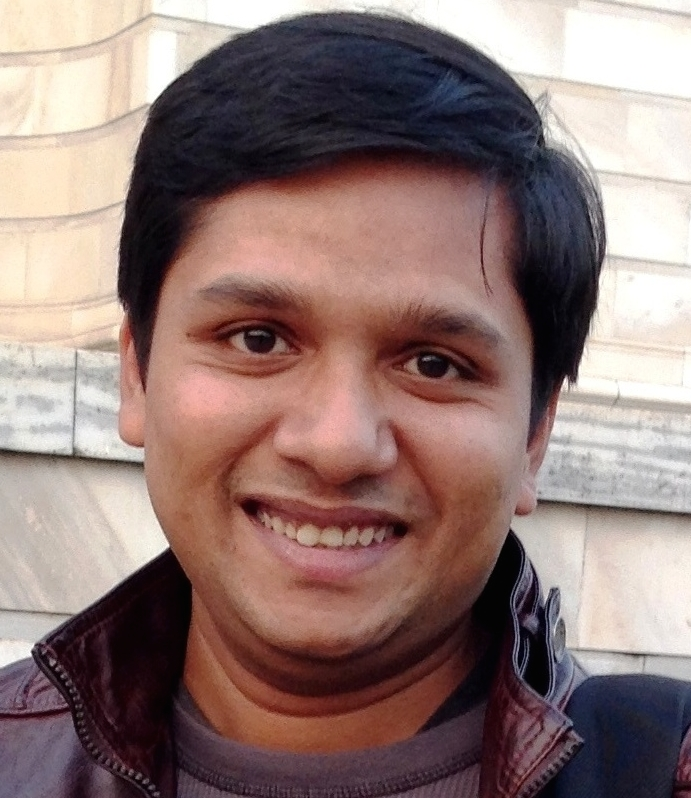
\includegraphics[height=1.25in]{Abhishek-Halder.jpg}}]{Abhishek
Halder}
(S'10-M'14) is an Assistant Professor in the Department of Applied Mathematics,
and is an affiliated faculty in the Department of Electrical and Computer Engineering at
University of California, Santa Cruz. Before that he held postdoctoral
positions in the Department of Mechanical and Aerospace Engineering at
University of California, Irvine, and in the Department of Electrical
and Computer Engineering at Texas A\&M University. He obtained his
Bachelors and Masters from Indian Institute of Technology Kharagpur in
2008, and Ph.D. from Texas A\&M University in 2014, all in Aerospace
Engineering. His research interests are in stochastic systems, control
and optimization with application focus on large scale cyber-physical
systems.
\end{IEEEbiography}

% You can push biographies down or up by placing
% a \vfill before or after them. The appropriate
% use of \vfill depends on what kind of text is
% on the last page and whether or not the columns
% are being equalized.

%\vfill

% Can be used to pull up biographies so that the bottom of the last one
% is flush with the other column.
%\enlargethispage{-5in}



% that's all folks
\end{document}


